\pagebreak
\section{Fazit}\label{sec:fazit}
\begin{figure}[H]
  \centering
  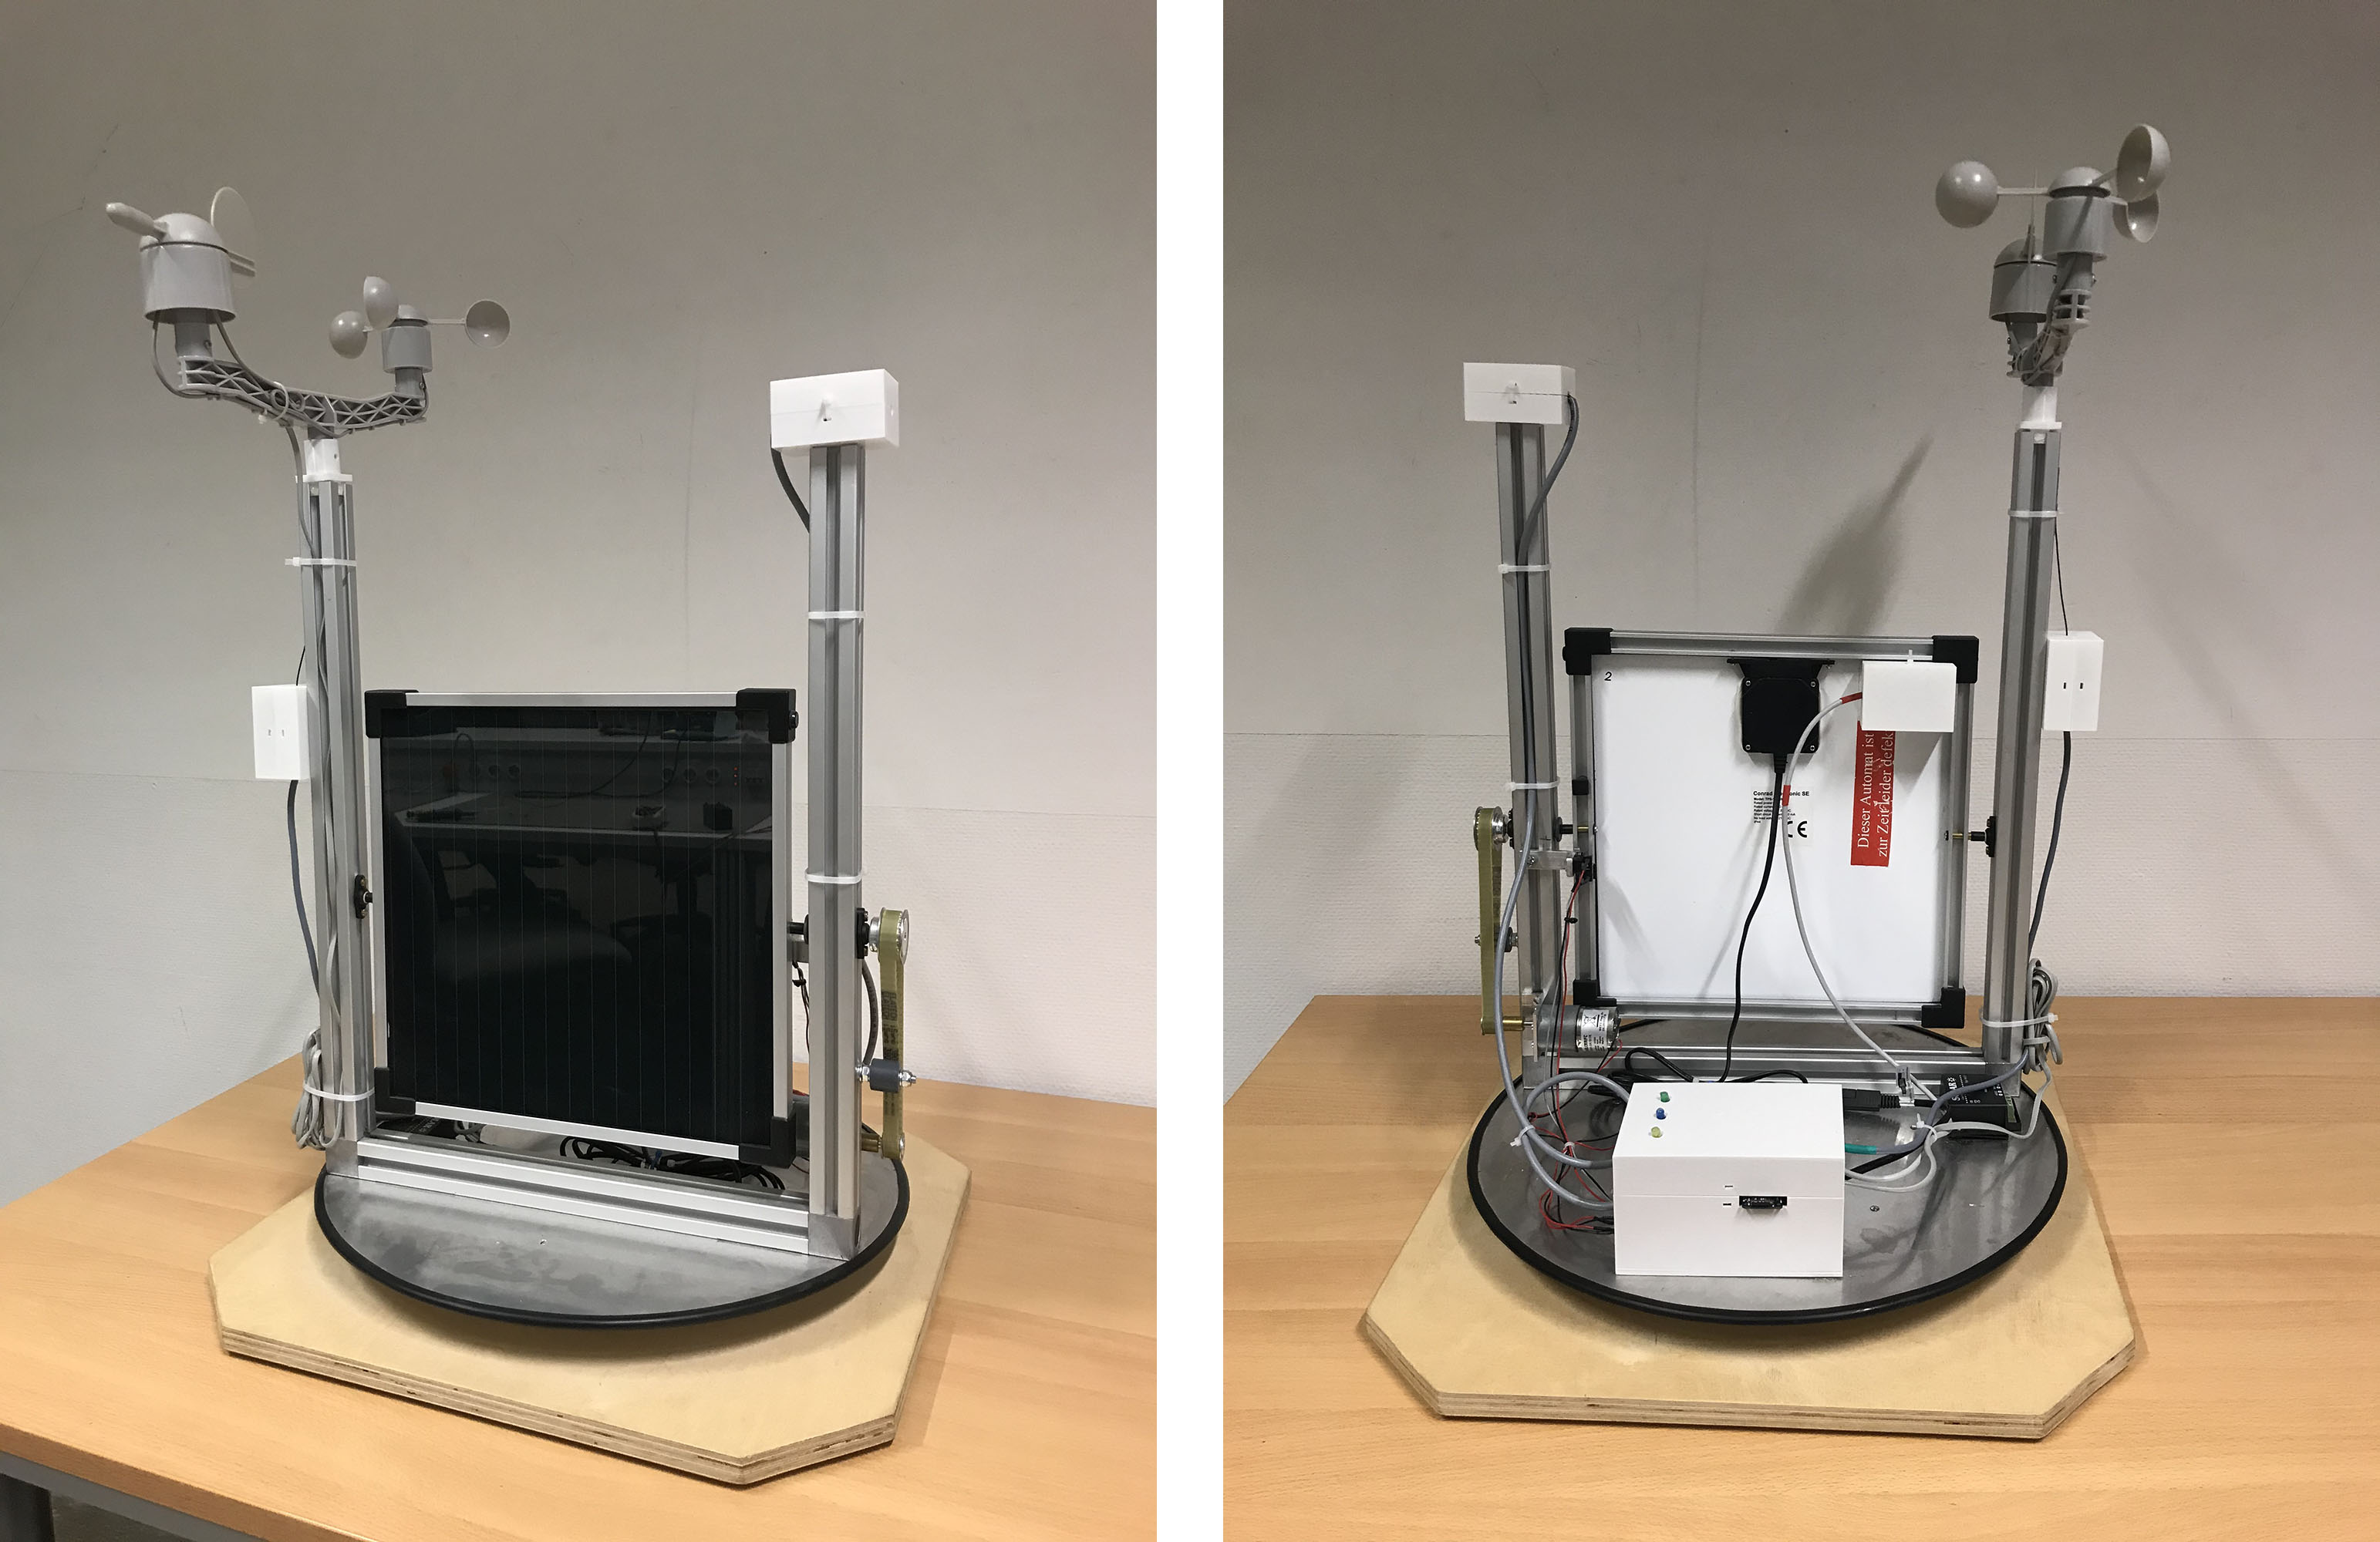
\includegraphics[width=0.8\textwidth]{./img/Wetterstaion_fertig1.jpg}
  \caption{Fertiggestellte Wetterstation}\label{fig.Wetterstationfertig}
\end{figure}

In Abbildung \ref{fig.Wetterstationfertig} wird der fertige Aufbau der Wetterstation dargestellt. Die Anforderung der Erfassung von Temperatur, Luftdruck und -feuchte wird mit dem BME280, der im Hauptgehäuse platziert ist, umgesetzt. Für die Erfassung von Windrichtung und -geschwindigkeit konnte ein neues Anemometer gefunden und implementiert werden.

Im Hauptgehäuse ließen sich Mikrokontroller, Platinen und Sensoren sinnvoll unterbringen (Abbildung~\ref{fig.hauptgehauese}). Die Wasserfestigkeit des Aufbaus konnte leider, mit den verfügbaren Mitteln, in der vorgegebenen Zeit, nicht erreicht werden. Das verwendete 3D-Druck-Material ist nicht für einen abgedichteten Aufbau geeignet. 


\begin{figure}[H]
  \centering
  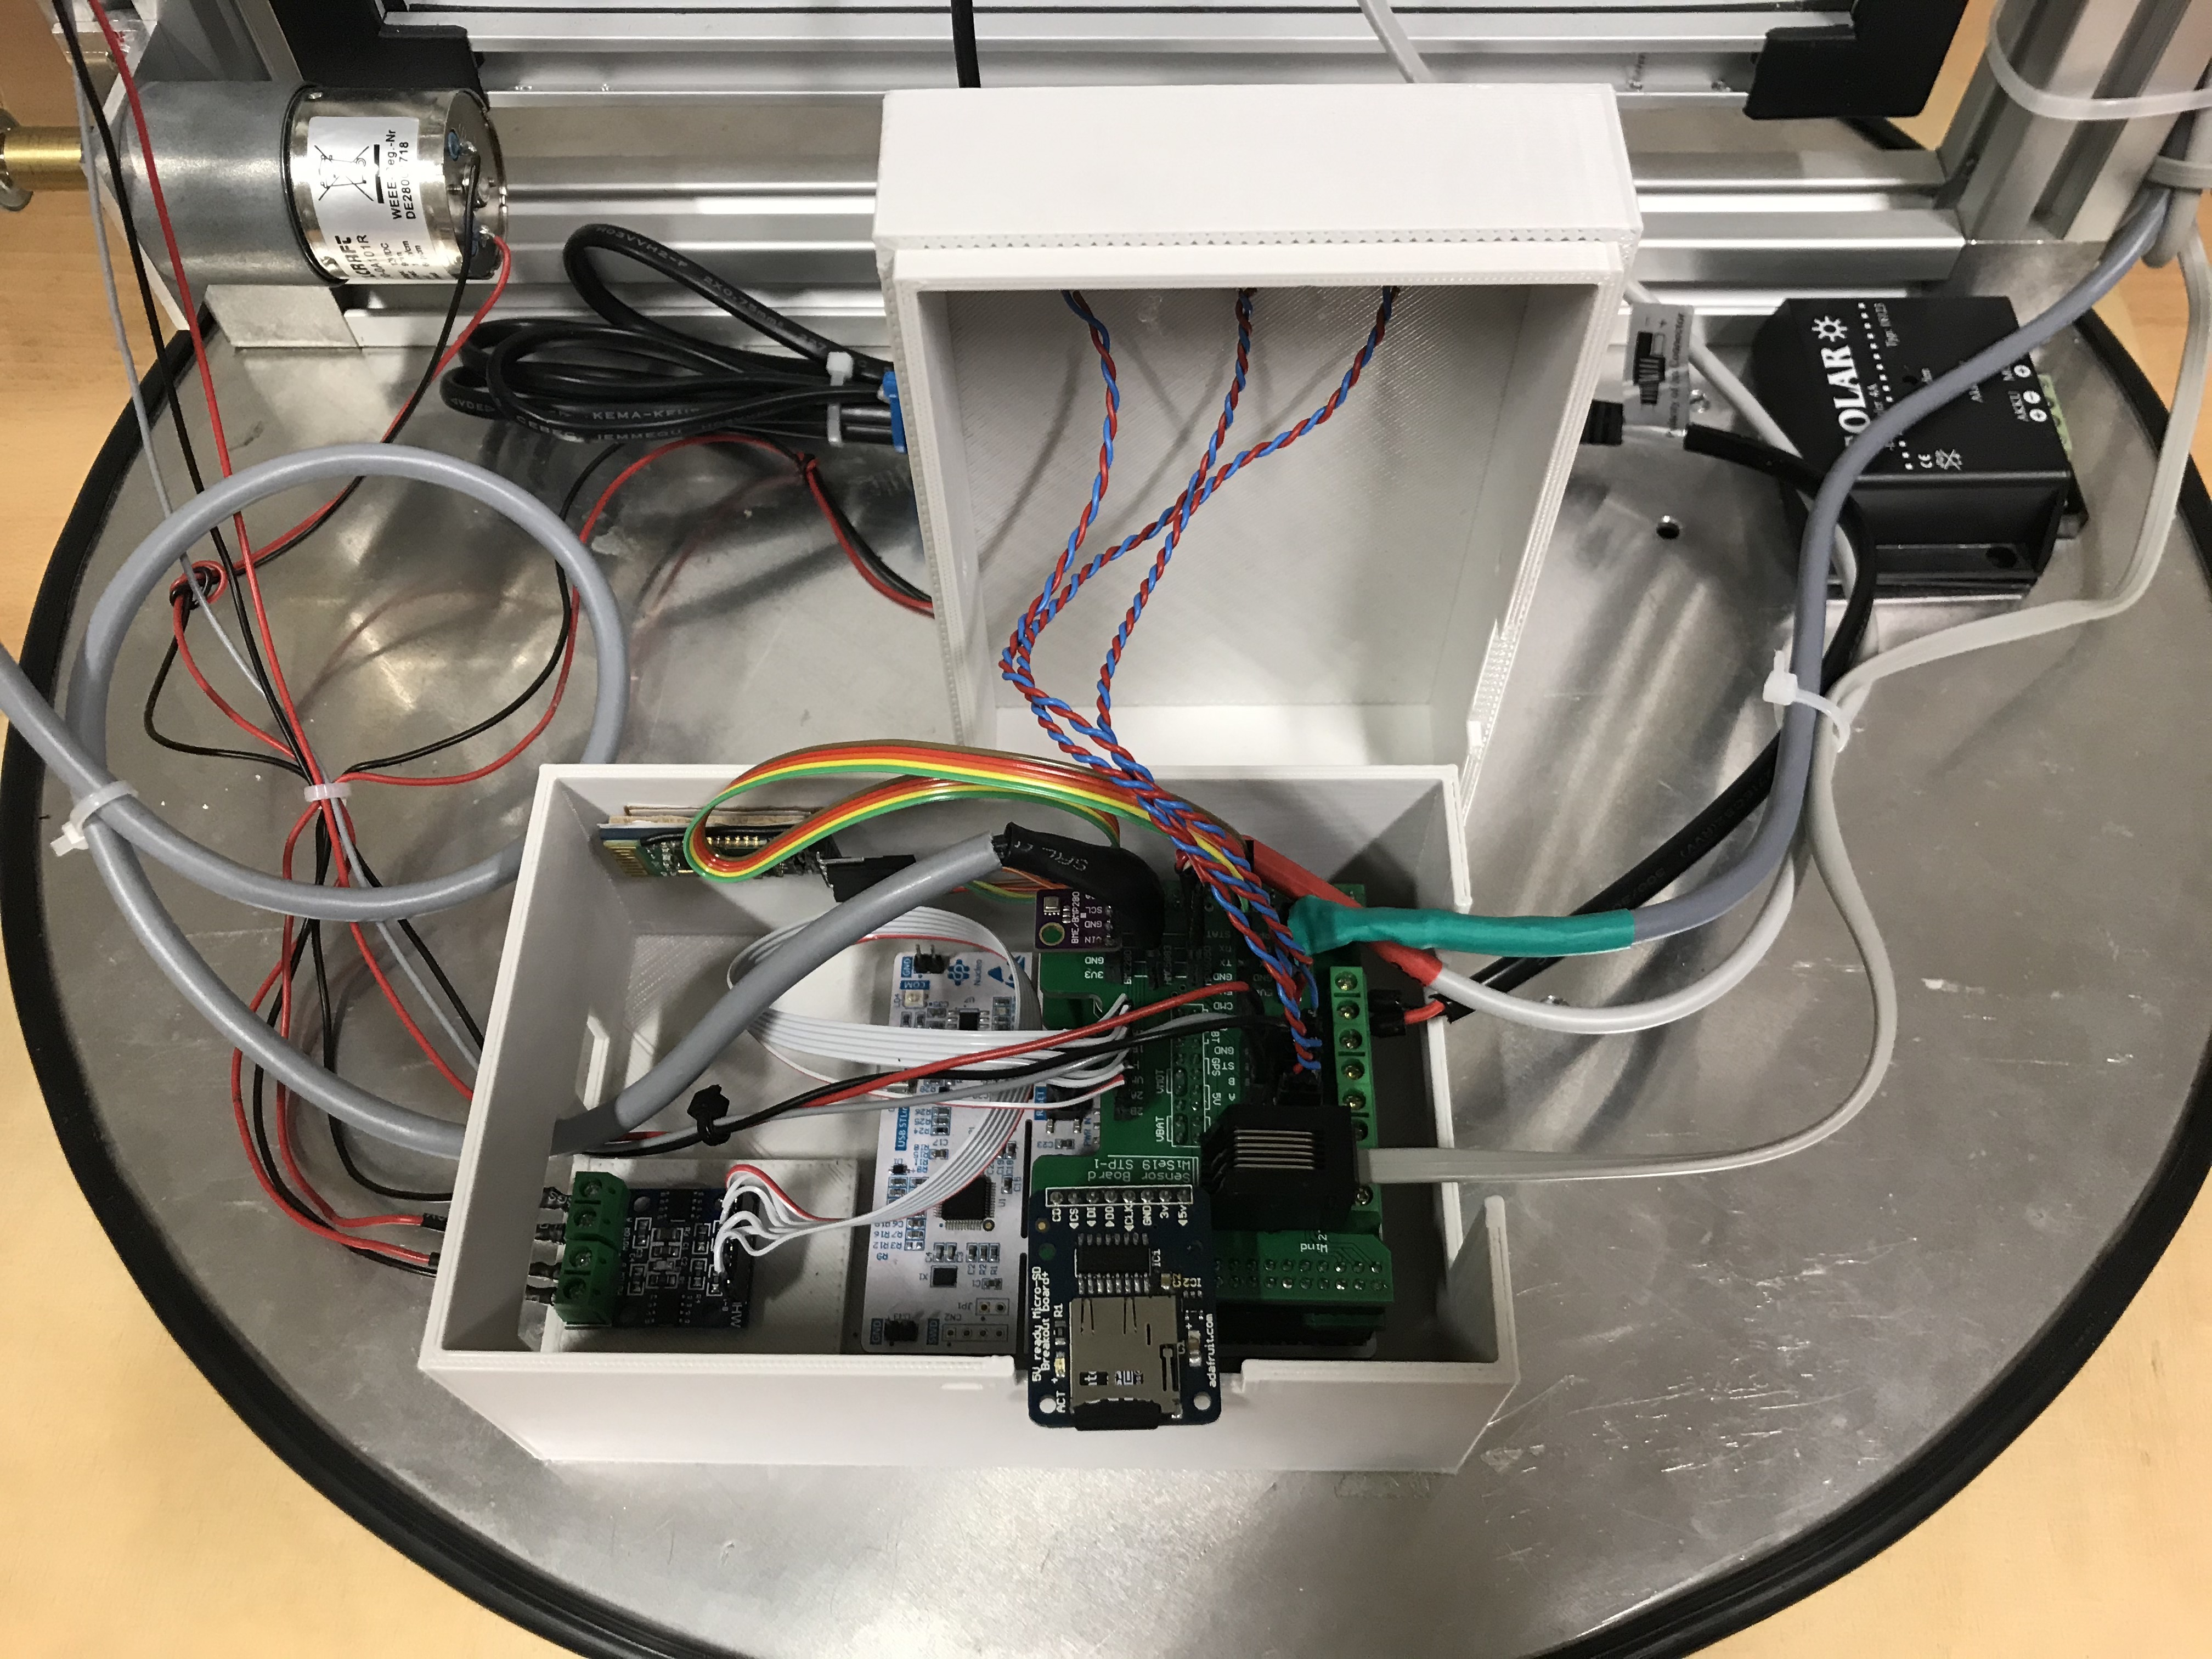
\includegraphics[width=0.7\textwidth]{./img/Hauptgehauese.jpg}
  \caption{Blick in das Hauptgehäuse}\label{fig.hauptgehauese}
\end{figure}

Sowohl hardware- als auch softwareseitig wurden verschiedene Energiesparmaßnahmen implementiert. Die letztendliche Laufzeit müsste noch in einem Langzeittest ermittelt werden. Der verbaute Neigungssensor wird letztendlich nicht zur Kompensation bei der Ausrichtung des Panels benutzt, ist aber in diesem Fall auch nicht nötig, da die Funktionalität trotzdem gegeben ist. Die Aufhängung des Panels ließe sich in ihrer Mechanik noch verbessern, da sie in ihrer aktuellen Umsetzung relativ instabil ist, sodass das Panel leicht schief hängt. Diese Verbesserung war jedoch im vorgegebenen Zeitrahmen nicht möglich.

Grundlegend lässt sich sagen, dass alle gegebenen Anforderungen an das Projekt erfüllt wurden. Zusätzlich wurde eine Benutzeroberfläche zum Bedienen der Wetterstation und Anzeigen der Messwerte entwickelt.



%%% Local Variables:
%%% mode: latex
%%% TeX-master: "../termpaper"
%%% End:
